The Analysis portion is how teams show that their requirements are verified and how they track any external analysis done to generate requirements. Figure \ref{fig:Analysis Organization} shows the top level organizational structure. As is the case throughout this Reference Architecture, many of the included packages are hyperlinked to more detailed diagrams. 

The Trade Studies package is a place to store any applicable trade studies in block form. This allows for requirements to be traced to any relevant analysis done in other tools. For example, if a team performed a Launch Vehicle Trade Study that ultimately impacted a requirement, that requirement could be traced to the Launch Vehicle Trade Study block, which includes the most current trade study as an attachment. This makes it very easy to know exactly where the numbers or decisions came from and stores that in the model for easy reference and modification from the team.

\begin{figure}[H]
    \centering
    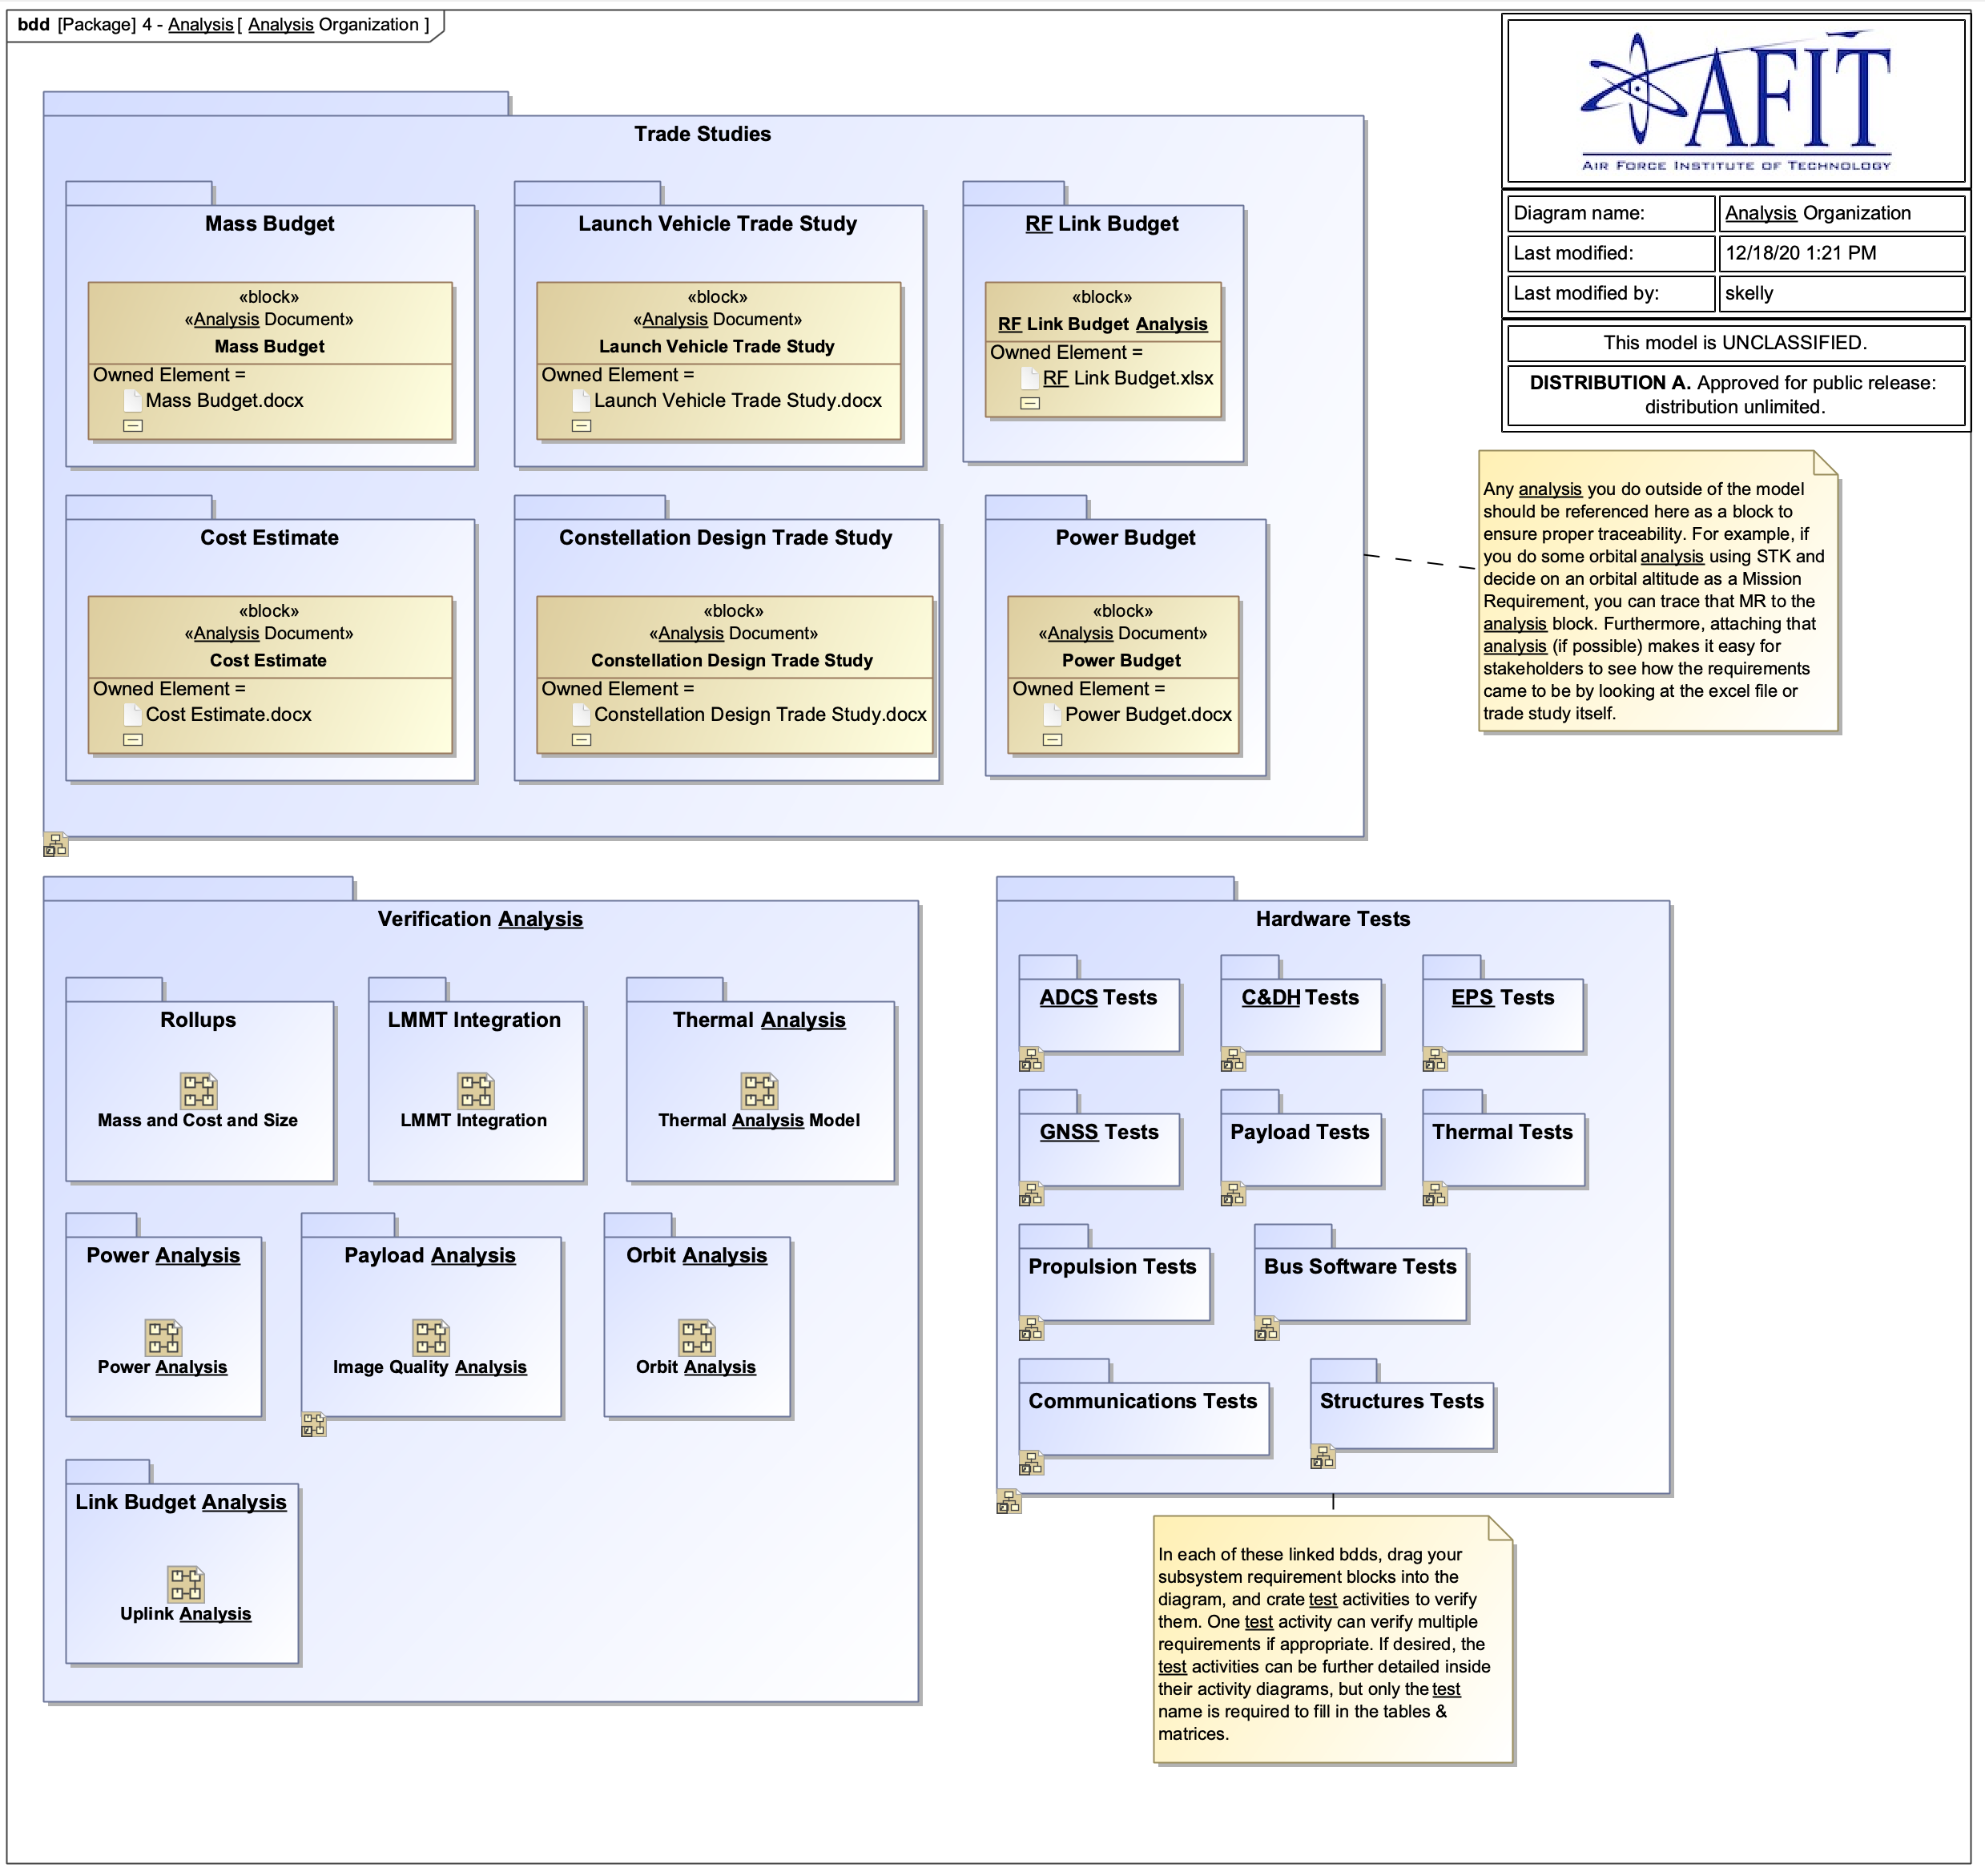
\includegraphics[width=\textwidth]{Thesis/Analysis_and_Results/Analysis and Results Figures/Analysis Organization.png}
    \caption{Analysis Organization}
    \label{fig:Analysis Organization}
\end{figure}

The Verification Analysis package contains several templates or patterns that highlight some capabilities of Cameo for requirement verification. For example, the Thermal Analysis parametric diagram in Figure \ref{fig:Thermal Analysis} shows how to use a MATLAB script to perform analysis based off the values entered in the thermal subsystem, as well as any other values that affect these calculations, such as the CubeSat's mass and some orbital parameters. The code in Figure \ref{fig:Thermal Analysis} is not necessary to read in this thesis, and is usually hidden from view when scripts become lengthy, but is shown here just to highlight where the code is stored. This section is intended to encourage teams to perform analysis within the model instead of in other tools. By performing analysis within the model, easy verification of candidate systems can be accomplished using Instance Tables or the default values assigned to component value properties. The CubeSat Reference Architecture purposefully does not include default values for the components' value properties, but an instance table, such as the one in Figure \ref{fig:Thermal Analysis Instances}, can be simulated using the MATLAB code to compare how different candidate systems perform. This instance was simulated, and the results are shown in Figure \ref{fig:Thermal Analysis Completed}. By changing one or several value properties in the relevant blocks or in the instance table, these graphs automatically update to show how the performance changes. This is extremely useful for many requirements that are affected by multiple subsystems or multiple components. A constraint block can be created that uses those value properties as inputs, and the performance outputs can be quickly assessed in multiple system configurations. The included parametric diagrams serve as patterns to replicate and modify, reducing the learning curve for teams who haven't learned these capabilities yet. 

\begin{figure}[H]
    \centering
    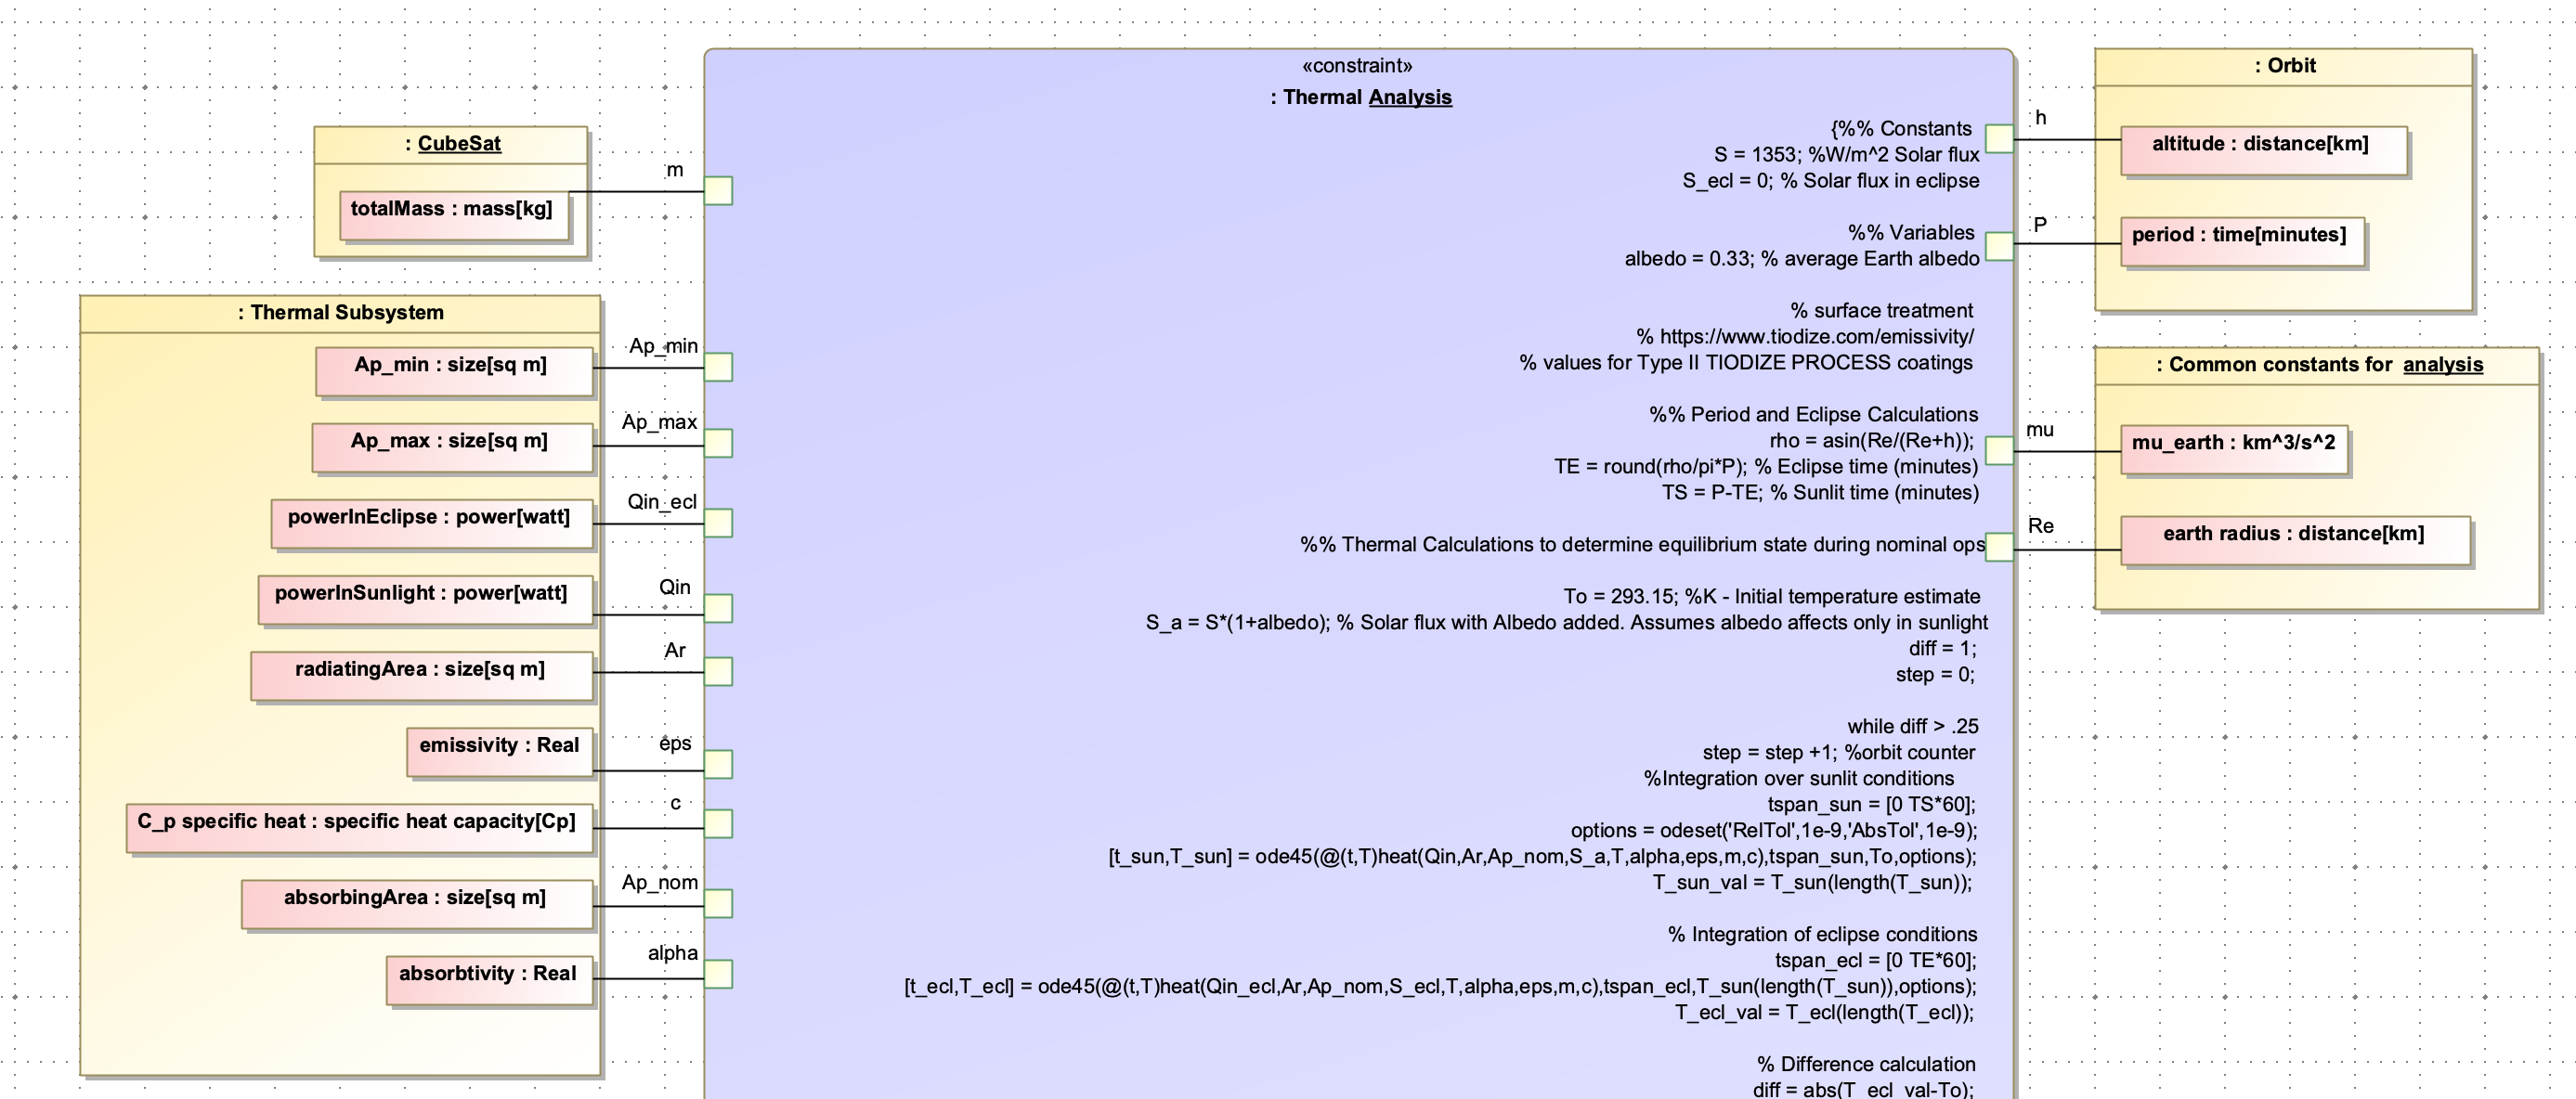
\includegraphics[scale=0.4, angle=90]{Thesis/Analysis_and_Results/Analysis and Results Figures/Thermal Analysis.png}
    \caption{Thermal Analysis}
    \label{fig:Thermal Analysis}
\end{figure}

\begin{figure}[H]
    \centering
    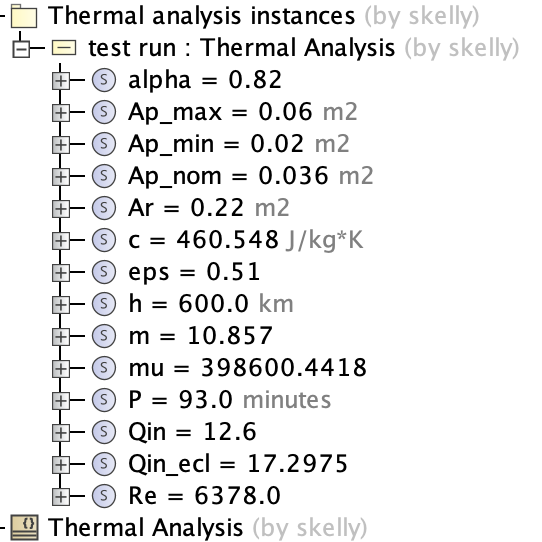
\includegraphics[width=4 in]{Thesis/Analysis_and_Results/Analysis and Results Figures/Thermal Analysis Instances.png}
    \caption{Thermal Analysis Instance}
    \label{fig:Thermal Analysis Instances}
\end{figure}

\begin{figure}[H]
    \centering
    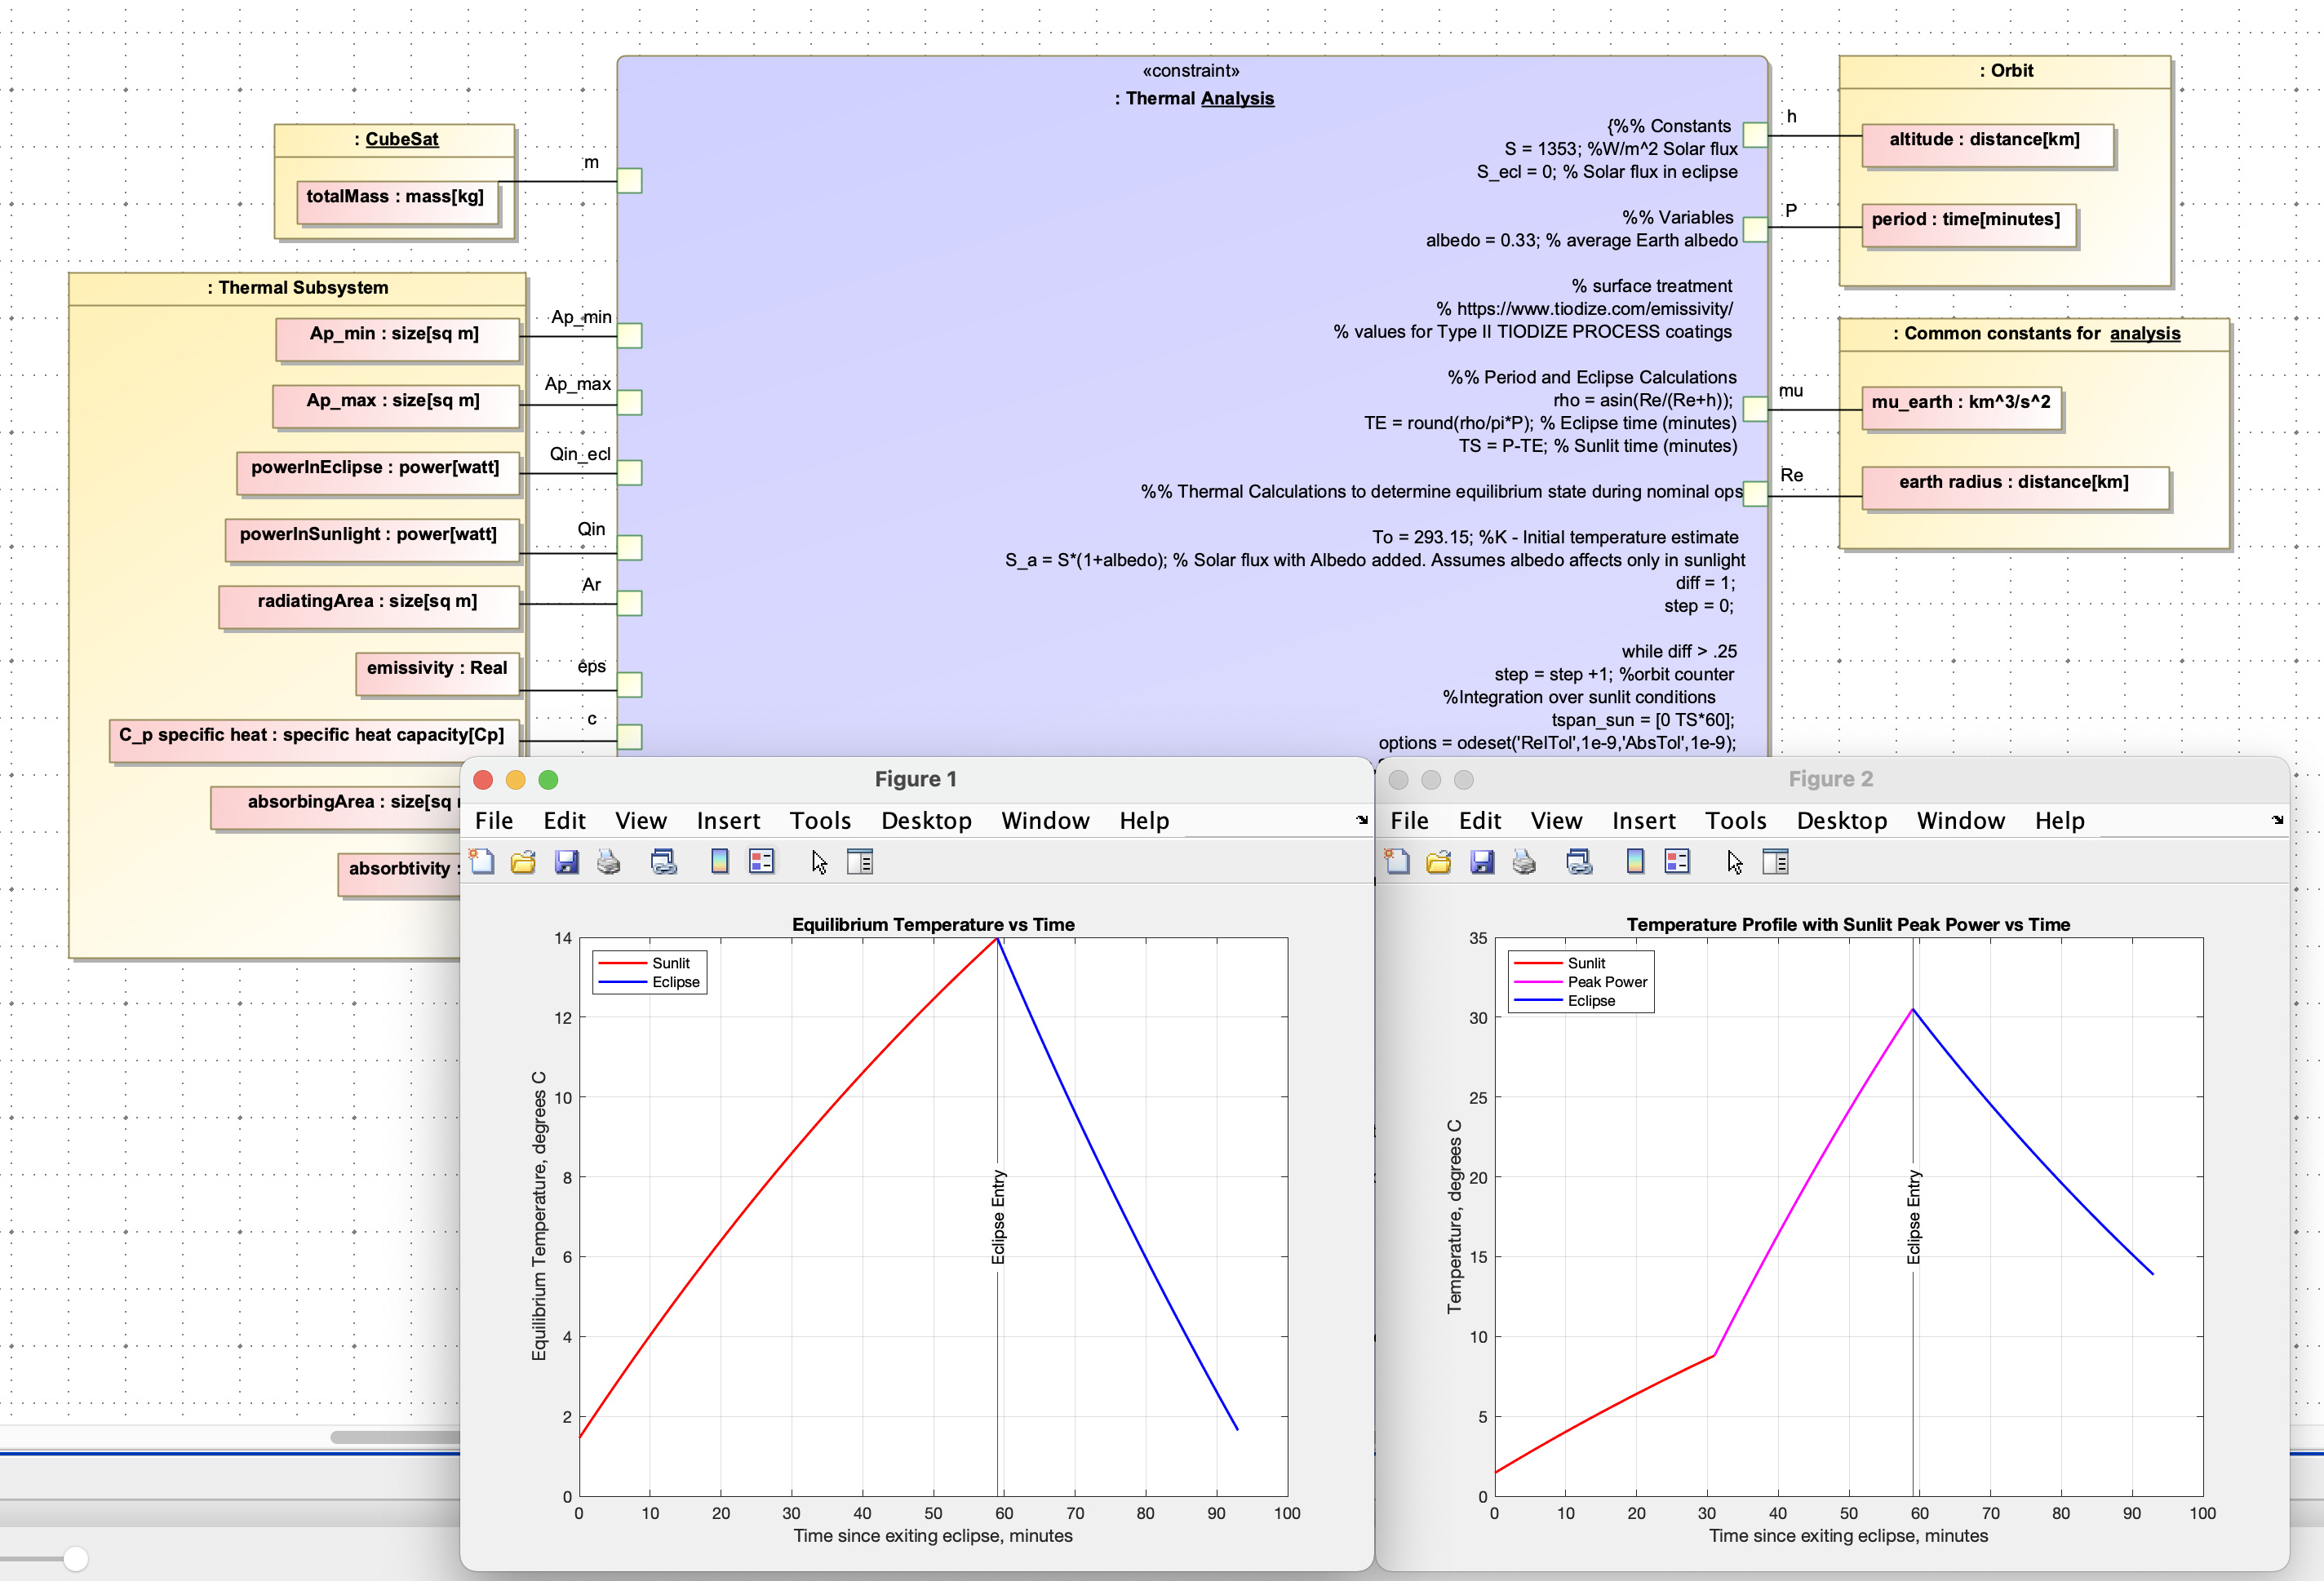
\includegraphics[scale=0.4, angle=90]{Thesis/Analysis_and_Results/Analysis and Results Figures/Thermal Analysis Run.png}
    \caption{Thermal Analysis Run}
    \label{fig:Thermal Analysis Completed}
\end{figure}

As teams progress from the design, they will test physical hardware. Before teams begin testing physical hardware though, they need to document their test plans. The Hardware Tests package includes workspaces for each subsystem that establishes consistency and makes it easier to generate the necessary tables to describe test activities. Each requirement should be tied to a test (sometimes multiple requirements can be verified by one test), and this can be done in diagram form. For example, if the \abbreviationFull[Electrical Power System]{EPS} lead needs to plan EPS testing activities, they can open up the EPS Tests bdd and follow the template process. If they drag and drop all of the applicable subsystem requirements onto this diagram, as shown in Figure \ref{fig:EPS Tests}, they can easily create test activities and assign a "verify" relationship between them, which automatically populates the included tables. In this example, notice the “Weigh Components” test, and that test verifies the EPS Subsystem Mass requirement. This pattern should be continued until each requirement is verified by some activity. Finally, the test activity tables provide a place to textually describe what happens in each test to verify the requirement(s). These tables are all useful for the Test Plans and Test Reports, keeping the model as the primary document instead of different files and formats for each subsystem. The subsystem requirement tables in this section also include a method for tracking testing progress while also establishing a common set of definitions. Previously, tests that were "not verified" for whatever reason were all in one category, causing confusion amongst stakeholders. Now, tests can be labeled from a drop-down menu as "not verified" for the specific reason and they are labeled in a color to bring attention to problematic tests. Figure \ref{fig:EPS Test Verification} shows an example of how this could be used. The Verification Status legend is located in the Component Library and can be modified if definitions or categories change.

\begin{figure}[H]
    \centering
    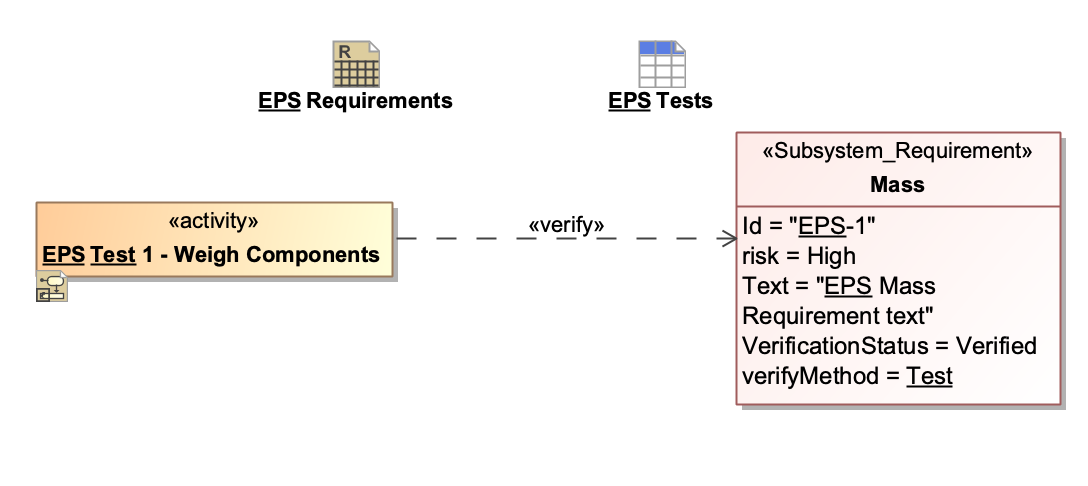
\includegraphics[width=\textwidth]{Thesis/Analysis_and_Results/Analysis and Results Figures/EPS tests.png}
    \caption{EPS Tests}
    \label{fig:EPS Tests}
\end{figure}

\begin{figure}[H]
    \centering
    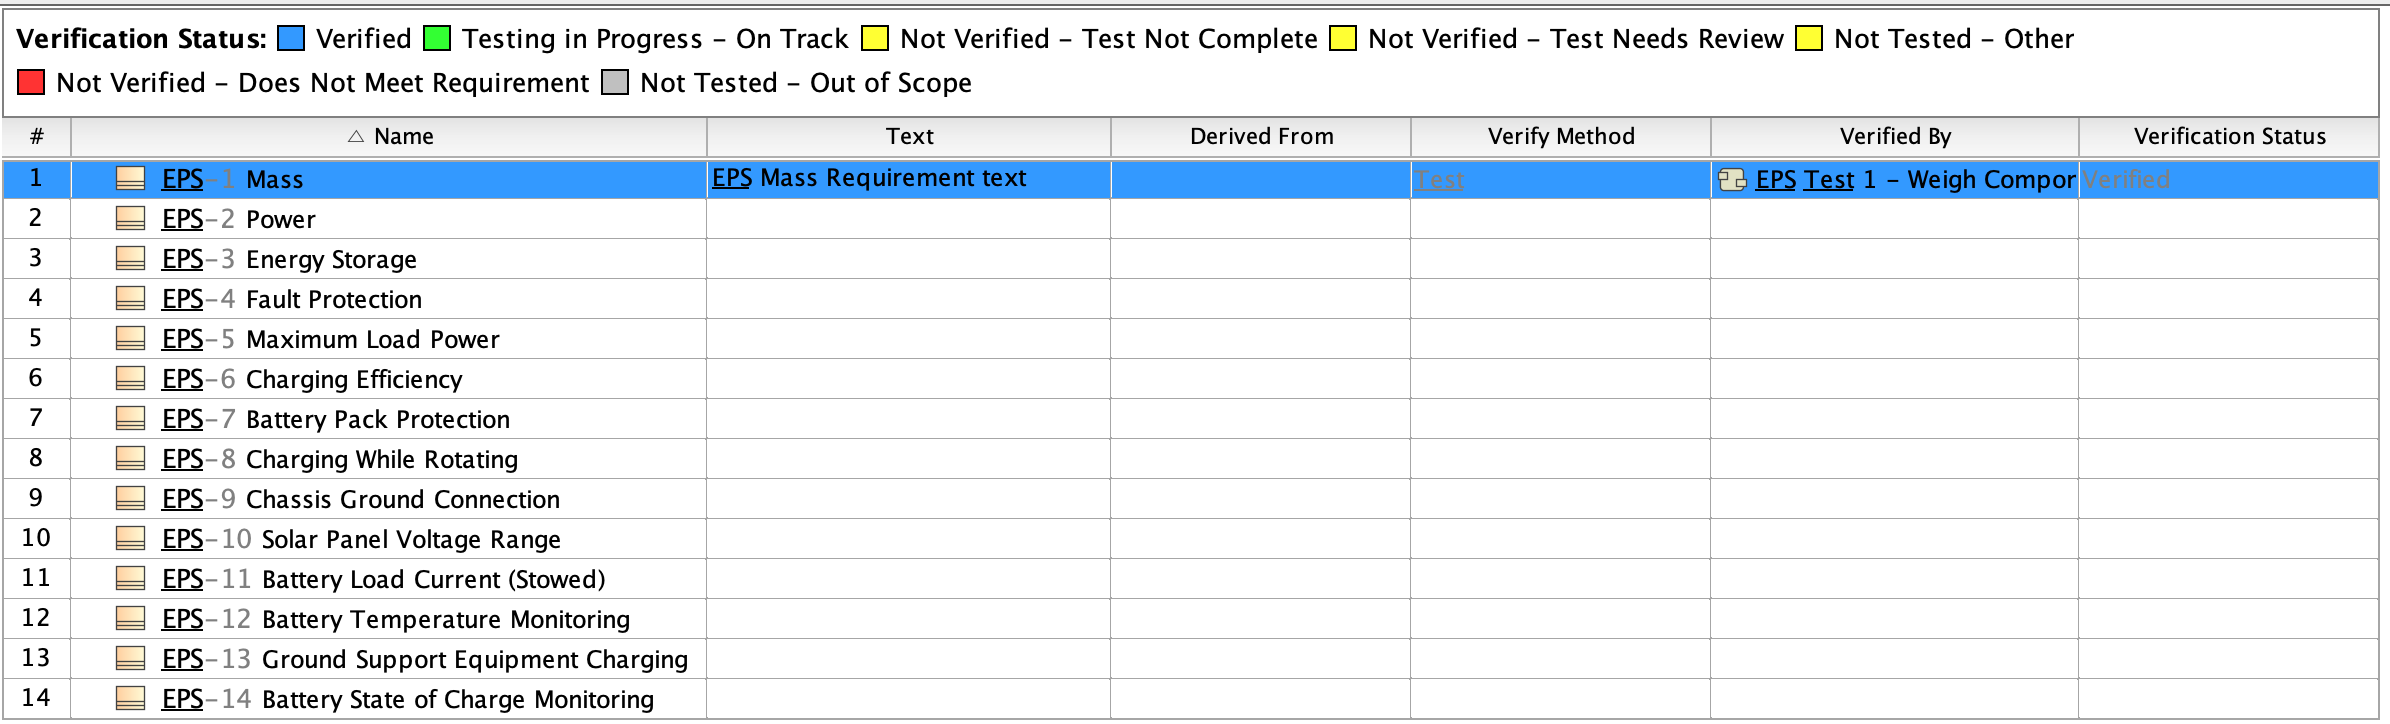
\includegraphics[width=\textwidth]{Thesis/Analysis_and_Results/Analysis and Results Figures/EPS Test Verification.png}
    \caption{EPS Test Verification}
    \label{fig:EPS Test Verification}
\end{figure}